\chapter[Projeto Eletrônico]{Projeto Eletrônico}

\section{Objetivo Específico}

Captar, condicionar e processar os dados obtidos através dos sensores internos e externos de um motor a combustão (FIAT 1.0 MPI), além de transmiti-los de forma precisa e sistematizada de acordo com requisitos não funcionais do SBAM (Software da Bancada de Análise de Motor)

\section{Requisitos}

Os principais parâmetros de um motor a serem avaliados são:

\begin{itemize}
	\item Temperatura do óleo do motor;
	\item Temperatura do ar no coletor de admissão;
	\item Pressão do ar no coletor de admissão;
	\item Velocidade angular do eixo das árvores de manivelas;
	\item Posição angular da válvula borboleta;
	\item Fluxo de ar posterior a válvula borboleta;
	\item Quantidade de oxigênio presentes nos gases de exaustão;
	\item Temperatura de entrada da água no radiador;
	\item Temperatura de saída da água no radiador;
	\item Temperatura dos gases de combustão.
\end{itemize}

A relação da temperatura da água na entrada e na saída do radiador apresenta a relação da transferência de calor entre motor e radiador.

Todos estes sensores são passivos e emitem os dados em forma de sinais elétricos, sendo eles, alguma relação de tensão e corrente de acordo com o parâmetro a ser monitorado. Como um dos requisitos deste projeto apresenta uma interação com um software, todos estes dados devem ser processados digitalmente, o que implica na utilização de um microcontrolador para a aquisição e processamento destes sinais e transmissão dos mesmos, de modo que o software possa interpretá-lo de forma fiel e precisa. 

O sinal que varia mais rapidamente em relação ao tempo é a velocidade angular das árvores de manivelas ou simplesmente o RPM (rotação por minuto) do motor, pois os sinais de temperatura e posição angular da válvula borboleta não variam tão rapidamente. O motor a ser analisado apresenta rotação máxima entre 6000 e 7000 rpm, transcrevendo isto para o domínio da frequência significa que a frequência máxima lida pelo sensor é de aproximadamente: 7000 rotações a cada 60 segundos.

\begin{equation}
	f = \frac{7000}{60} \cong 117 Hz	
\end{equation}

Com isso adotando-se o critério de \textit{Nyquist-Shanon} \cite{diniz2014processamento} a taxa mínima de amostragem deste sinal sem perda de informação é dada pelo dobro da frequência máxima do sinal amostrado, evitando o efeito de \textit{Aliasing} \cite{diniz2014processamento}. Portanto para estabelecer este critério o \textit{clock} mínimo do microcontrolador deve ser de 234 Hz.

Além disso tendo em vista que são ao total 10 sensores o microcontrolador deve ter ao menos 10 pinos GPIO (\textit {General Pruporse Inputs/Outpus}) para que o mesmo tenha acesso ao barramento com os dados do sensor. 

Por via de segurança é cabível que o usuário não esteja próximo ao motor no momento em que o mesmo esteja funcionando, portanto, uma aplicação via software para realizar a partida do motor, além do controle de velocidade, também abrange este projeto.

\section{Implementação}

Tendo em vista a quantidade de sensores a serem analisados e o estado crítico do controle do sistema de partida e aceleração do motor, cada um destes sistemas (aquisição de dados, controle) terá um microcontrolador dedicado que serão estruturados e organizados a partir de um servidor.

\subsection{Sistema de Aquisição}

Todo sistema de aquisição a ser implementado pode ser dividido em 4 módulos, apresentados na figura \ref{diagramaDeAquisicaoDeDados}

\begin{figure}[h!]
	\centering
	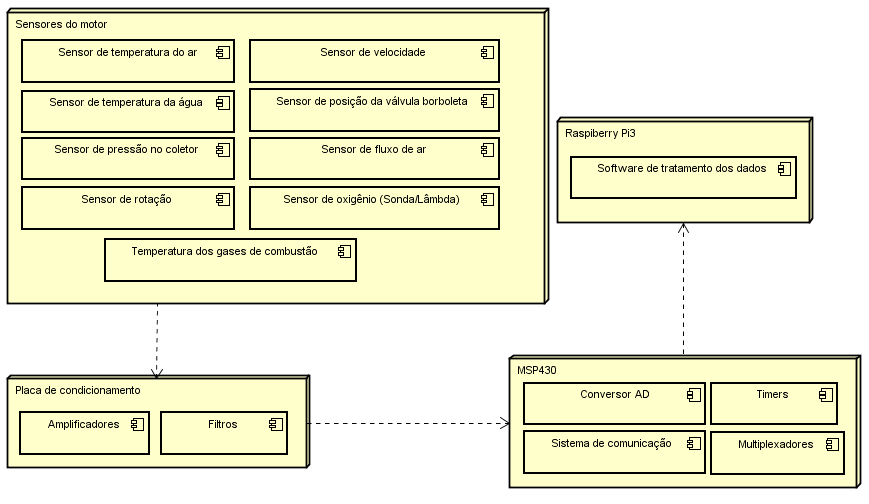
\includegraphics[keepaspectratio=true,scale= 1.0, angle=90]{figuras/Diagrama.PNG}
	\caption{Diagrama de aquisição de dados}
	\label{diagramaDeAquisicaoDeDados}
\end{figure}
\pagebreak

\subsubsection{Sensores}

Os sensores utilizados internamente no motor apresentam características específicas apresentadas na tabela \ref{PrincipaisSensoresInternosDeUmMotor}.

\begin{table}[h!]
	\centering
	\caption{Principais sensores internos de um motor}
	\label{PrincipaisSensoresInternosDeUmMotor}
	
	\begin{tabular}{|c|c|c|c|}
		\hline
		\textbf{Parâmetros}          & \textbf{\begin{tabular}[c]{@{}c@{}}Tipo de \\ Sinal Gerado\end{tabular}} & \textbf{Tipo de sensor}                                                                                    & \textbf{Descrição}                                                                                           \\ \hline
			Temperatura do óleo          & Analógico                     & Termopar Tipo K                                                                                            & \begin{tabular}[c]{@{}c@{}}Monitora a \\ temperatura do óleo \\ no motor\end{tabular}  \\ \hline
		Temperatura do ar            & Analógico                     & Termopar Tipo K                                                                                            & \begin{tabular}[c]{@{}c@{}}Monitora a\\ temperatura do ar no\\ coletor de admissão\end{tabular}              \\ \hline
		Temperatura da Água          & Analógico                     & Termopar Tipo K                                                                                            & \begin{tabular}[c]{@{}c@{}}Monitora a \\ temperatura do líquido \\ de arrefecimento do\\ motor\end{tabular}  \\ \hline
		Pressão no Coletor           & Analógico                       & Pressão diferencial                                                                                        & \begin{tabular}[c]{@{}c@{}}Monitora a pressão do\\  ar no coletor de \\ admissão\end{tabular}                \\ \hline
		Rotação                      & Digital                       & Sensor Indutivo                                                                                            & \begin{tabular}[c]{@{}c@{}}Mede velocidade \\ angular do eixo\\ das árvores de\\ manivelas\end{tabular}      \\ \hline
		Velocidade                   & Digital                       & Sensor Indutivo                                                                                            & \begin{tabular}[c]{@{}c@{}}Mede velocidade\\ angular do eixo\\  posterior a \\ transmissão\end{tabular}      \\ \hline
		Posição da válvula borboleta & Analógico                     & Potenciômetro Linear                                                                                       & \begin{tabular}[c]{@{}c@{}}Monitora a posição\\ angular da válvula\\  borboleta\end{tabular}                 \\ \hline
		Fluxo de Ar                  & Analógico                     & Potenciômetro Linear                                                                                       & \begin{tabular}[c]{@{}c@{}}Monitora o fluxo\\ de ar posterior\\ a válvula borboleta\end{tabular}             \\ \hline
		Oxigênio (Sonda/Lambda)      & Analógico                     & \begin{tabular}[c]{@{}c@{}}Eletrodos de platina \\ separados por óxidos\\  ativos TiO2 e ZrO2\end{tabular} & \begin{tabular}[c]{@{}c@{}}Monitora a quantidade\\ de oxigênio presente\\ nos gases de exaustão\end{tabular} \\ \hline
	\end{tabular}
\end{table}

\clearpage

\begin{table}[h!]
	\centering
	\caption{Sensores a serem implementados. Fonte: Autores}
	\label{SensoresASeremImplementados}
	\begin{tabular}{|l|l|l|l|}
		\hline
		\textbf{Parâmetros}                                                                     & \textbf{\begin{tabular}[c]{@{}l@{}}Tipo de \\ Sinal Gerado\end{tabular}} & \textbf{Tipo de Sensor} & \textbf{Descrição}                                                                                                  \\ \hline
		\begin{tabular}[c]{@{}l@{}}Temperatura de\\ entrada da água no\\  radiador\end{tabular} & Analógico                                                                & Termopar (K)         & \begin{tabular}[c]{@{}l@{}}Monitora a \\ temperatura de entrada\\ da água no radiador\end{tabular}                  \\ \hline
		\begin{tabular}[c]{@{}l@{}}Temperatura de \\ saída da água \\ no radiador\end{tabular}  & Analógico                                                                & Termopar (K)         & \begin{tabular}[c]{@{}l@{}}Monitora a \\ temperatura da água \\ na saída do radiador\end{tabular}                   \\ \hline
		\begin{tabular}[c]{@{}l@{}}Temperatura dos\\ gases de \\ Combustão\end{tabular}         & Analógico                                                                & Termopar Tipo K         & \begin{tabular}[c]{@{}l@{}}Monitora a \\ temperatura dos \\ gases de combustão\\  no sistema de escape\end{tabular} \\ \hline
	\end{tabular}
\end{table}

\begin{itemize}	
	\item \textbf{Termopar Tipo K}: É um sensor utilizado para a medição de temperatura. Ele é feito utilizando dois metais diferentes ligados por suas extremidades. Quando há uma diferença de temperatura entre a extremidade unida e as extremidades livres, verifica-se o surgimento de uma diferença de potencial que pode ser medida por um voltímetro. Normalmente a saída é dada em microvolts, por isso, faz-se necessário o uso de uma placa de condicionamento para amplificação desse sinal. Nesse projeto, foi escolhido esse sensor devido a sua capacidade de ler uma faixa de temperatura entre 0 e 1240$º$C, além disso, por sua construção física permite a leitura de temperatura em meios fluidos. Necessária para essa aplicação \cite{vdo01}.
	
	\item \textbf{Sensor Indutivo}: Fornece ao módulo um sinal elétrico que possibilita a medição do número de rotação. O sinal gerado pelo sensor é obtido pela variação do fluxo magnético. Com a rotação do motor, os dentes da roda dentada passam pelo sensor e este fornece um sinal de tensão a cada passagem dos dentes ou ressaltos. Este sensor já é um ítem embutido no motor utilizado no projeto\cite{vdo01}.
	
	\item \textbf{Potênciometro Linear}:
	Utilizado para captar a posição da válvula borboleta o potênciometro atua na variação da resistência de acordo com a variação da posição de um eixo que é rotacionado Escolhido para esse projeto pois se adequa com simplicidade à variação de posição que se deseja obter para permitir análise de dados nessa bancada\cite{vdo01}.
	
	\item \textbf{Pressão Diferencial}: 
	Sensor MPX5700D é um sensor de pressão designado a para aplicações da largos ranges de pressão, atuando em pressões entre 0 e 700 kPa. Produz na sua saída níveis de tensão de 0.2 a 4.7 V, o que implica a não necessidade de um condicionamento do sinal.
\end{itemize}

\subsubsection{Microcontrolador}

Analisando os tipos de sensores das tabelas \ref{PrincipaisSensoresInternosDeUmMotor} e \ref{SensoresASeremImplementados}, levando em consideração os tipos de sinais de saída e a quantidade de parâmetros a serem analisados, o microcontrolador selecionado para realizar a aquisição e processamento destes sinais foi a MSP430 (\textit{Texas Instruments}), pois esta apresenta as seguintes características relevantes para este projeto \cite{texas01}:

\begin{itemize}
	\item 8 portas I/O digitais;
	\item \textit{Clock} principal 16 MHz, posibilitando um tempo hábil para processamento de instruções e sinais;
	\item 2 conversores A/D, sendo 1 de 10 bits e 1 de 12 bits;
	\item Baixo consumo de energia, sendo da ordem de $\mu$W (micro Watts) atuando no modo de baixo consumo;
	\item Portas configuráveis como UART, o que possibilita a utilização de um protocolo de comunicação serial.
\end{itemize}

A análise para seleção do microcontrolador foi feita baseada nos requisitos determinados anteriormente e o custo do dispositivo, tendo em vista que para a implementação do projeto a MSP430 já era um dos recursos disponíveis, sendo então necessária apenas a análise com relação à demanda dos requisitos. 

Este microcontrolador atua com níveis de tensão 0 - 3.3V, entretanto, alguns dos sensores apresentam níveis de tensão muito baixo, na ordem de $\mu$V, o que dificulta o tratamento destes sinais, onde há grande probabilidade de erro de leitura, levando em consideração ruídos e interferências. Com isso, faz-se necessária a implementação de um circuito de condicionamento de sinais, amplificando sinais muito baixos e removendo os ruídos, para assim então realizar uma leitura mais precisa no microcontrolador.

\subsubsection{Placa de condicionamento}

O condicionamento do sinal de saída dos sensores é necessário para poder interfaceá-lo com os outros elementos do sistema e tornar assim, sua leitura compreensível para o usuário.

O condicionamento de sinal passa por várias etapas: amplificar, filtrar e equalizar o sinal para que este ganhe níveis de tensão adequados, com boa relação sinal/ruído e distorção harmônica mínima. A aquisição do sinal analógico culmina na sua amostragem e posterior conversão analógica digital (A/D) \cite{SMAR}.

De acordo com estudos apresentados pela National Instruments \cite{national01}, condicionar um sinal consiste em: amplificar, atenuar, excitar, isolar, filtrar, linearizar, aplicar compensação de junção fria e a configuração de ponte. Porém a maioria dos sensores necessitam somente de amplificação, isolação, filtragem, linearização e excitação, dependendo do seu comportamento.

Abaixo uma pequena contextualização quanto aos conceitos que mais são utilizados com os tipos de sensores deste aplicação:

\begin{itemize}
	\item Amplificação: Consiste no aumento do nível de tensão para alcançar a faixa em que o conversor ADC atua, aumentando assim a sensibilidade e resolução do sinal lido. Com exemplo de circuito na Fig \ref{amplificadorDeInstrumentacao}.
	\item Isolação: É necessária para que o sinal provindo do sensor não ocorra de danificar o resto do sistema. “Separa” fisicamente o dispositivo de medição, utilizando técnicas como, transformadores, acopladores óticos ou capacitivos.
	\item Filtragem: Os filtros rejeitam ruídos indesejados dentro de uma determinada faixa de frequência, podendo ser adicionado ao circuito um filtro passa-baixas, passa-altas, passa-faixas ou até mesmo um filtro anti-aliasing, para bloquear ruídos de frequências indesejadas ou para atenuar sinais acima da frequência de \textit{Nyquist}
	\item Linearização: Quando os sensores produzem sinais de tensão ou corrente que não são linearmente relacionados com a medição física, é preciso linearizar este sinal. Estes processo podendo ser realizado por meio de condicionamento físico do sinal ou por software.
\end{itemize}

\begin{figure}[h!]
	\centering
	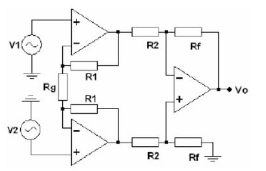
\includegraphics[keepaspectratio=true,scale= 0.7]{figuras/Amplificador.PNG}
	\caption{Amplificador de Instrumentação \cite{SMAR}}
	\label{amplificadorDeInstrumentacao}
\end{figure}

Na figura \ref{amplificadorDeInstrumentacao} é representado um modelo de amplificador de instrumentação, constituído em um circuito de ganho definido pelas relações entre as resistências. A tensão de saída é definida pela diferença de potencial entre as entradas e o ganho relacionado às resistência. Tal cálculo pode ser deduzido pela análise nodal junto das propriedades de amplificadores operacionais, sobre as tensões nas entradas e a relação com a saída.

\subsection{Sistema de Controle}

O controle do sistema é realizado de forma semelhante à mostrada na Figura \ref{CadeiaDeMedicao}. Os sensores e atuadores são conectados no motor para realizar as medições. 

No caso da medição, somente a leitura do valor da saída do sensor não é suficiente para completa leitura por parte do microcontrolador. Para isso é necessário o condicionamento destes sinais, só assim, serão enviados para conversão analógica digital e processados pelo algoritmo de controle.

Na nossa aplicação é desejado o controle da aceleração e da ignição de forma eletrônica. Para isso temos o atuador que recebe um sinal condicionado do microcontrolador e realiza tarefa desejada. Em algumas situações o conversor de potência é requisitado, visto que o sinal fornecido pelo microcontrolador não tem amplitude suficiente para afetar o processo alvo.

\begin{figure}[h!]
	\centering
	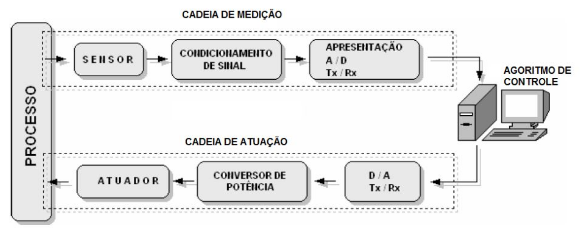
\includegraphics[keepaspectratio=true,scale= 0.9]{figuras/CadeiaDeMedicao.PNG}
	\caption{Cadeia de Medição e Atuação em Sistemas de Controle \cite{SMAR}}
	\label{CadeiaDeMedicao}
\end{figure}

\subsection{Sistema de Comunicação}

\subsubsection{Protocolo de comunicação I$^{2}$C}

O protocolo I$^{2}$C possui dois tipos de dispositivos, \textit{Master} e \textit{Slave}. O \textit{Master} é a unidade responsável por coordenar todos os periféricos (\textit{Slaves}). Dessa maneira, \textit{Master} sempre verifica se existe um \textit{Slave} na rede e caso exista, ele responde, começando assim, a transferência de dados.
Neste projeto como é a raspberry Pi 3 que é responsável por realizar o processamento dos dados para gerar a informação final figura \ref{DiagramaDeAquisicaoDeDados}, é considerada então o \textit{Master}, pois é a raspberry a responsável por controlar o sistema de comunicação com ambas MSP430, tanto de controle, quanto a de aquisição.


\subsection{Custos}

A tabela \ref{tabelaCustos} apresenta os custos dos componentes a serem utilizados na parte eletrônica do projeto da bancada. Tais valores podem sofrer ajustes e foram consultados através dos links apresentados na tabela no período de 15 a 30 de março de 2017. 


\begin{table}[h!]
	\centering
	\caption{Custos dos componentes}
	\label{tabelaCustos}
	\begin{tabular}{|l|l|l|l|}
		\hline
		\textbf{Componente}                                                                             & \textbf{Preço(Unidade)} & \textbf{Quantidade} & \textbf{Loja: Links para consulta}                                                                                                                                                                        \\ \hline
		AD595                                                                                           & R\$:87,00               & 6                   & \begin{tabular}[c]{@{}l@{}}http://produto.mercadolivre.com.br/\\ MLB-712124692-ad595-thermocou\\ ple-amplifier-circuito-integrado-\_\\ JM?source=gps\end{tabular}                                         \\ \hline
		\begin{tabular}[c]{@{}l@{}}Sensor De \\ Pressão Mpx5700\end{tabular}                            & R\$ 60,00               & 6                   & \begin{tabular}[c]{@{}l@{}}http://produto.mercadolivre.com.br/\\ MLB-708718648-sensor-de-presso\\ -mpx5700-para-arduino-pic-e-etc-\_\\ JM?source=gps\end{tabular}                                         \\ \hline
		\begin{tabular}[c]{@{}l@{}}Kit para Placa de\\ Circuito Impresso\end{tabular}                   & R\$: 65,00              & 1                   & \begin{tabular}[c]{@{}l@{}}http://produto.mercadolivre.com.br/\\ MLB-715578391-kit-p-confecciona\\ r-placa-de-circuito-impresso-suekit\\ -ck-3-\_JM\end{tabular}                                          \\ \hline
		\begin{tabular}[c]{@{}l@{}}Placa de Circuito\\ Impresso\end{tabular}                            & R\$:11,39               & 2                   & \begin{tabular}[c]{@{}l@{}}http://www.huinfinito.com.br/plac\\ as-circuito-impresso/636-placa-fe\\ nolite-virgem-face-simples-20x20\\ cm.html?search\_query=circuito+i\\ mpresso\&results=12\end{tabular} \\ \hline
		MSP430                                                                                          & R\$:85,00               & 2                   & \begin{tabular}[c]{@{}l@{}}2http://produto.mercadolivre.com.\\ br/MLB-842870672-microcontro\\ lador-msp430-hercules-launchpad-\\ \_JM\end{tabular}                                                        \\ \hline
		RaspBerry Pi                                                                                    & R\$:189,98              & 1                   & \begin{tabular}[c]{@{}l@{}}http://produto.mercadolivre.com.br\\ /MLB-810455120-novo-raspberry\\ -pi-3-model-b-pi3-quadcore-12gh\\ z-top-\_JM\end{tabular}                                                 \\ \hline
		\begin{tabular}[c]{@{}l@{}}Termopar tipo K\\ (Temp. agua\\ radiador e \\ ambiente)\end{tabular} & R\$ 15,80               & 6                   & \begin{tabular}[c]{@{}l@{}}http://produto.mercadolivre.com.br\\ /MLB-835569184-termopar-tipo-k\\ -sonda-1-metro-ponta-rosca-6mm-\\ \_JM?source=gps\end{tabular}                                           \\ \hline
		Total                                                                                           & R\$: 460,16             & 125                 &                                                                                                                                                                                                           \\ \hline
	\end{tabular}
\end{table}
\newpage
\section{Materiais e Metodos}

\section{Descrição dos Componentes}
Alguns dos componentes tem sua descrição detalhada dispensável como a Protoboard, Jumpers, capacitores, microcontroladores e o adaptador para o C.I. que foi utilizado somente para acoplá-lo corretamente à protoboard e realizar testes antes de confeccionar o circuito final, vista a diferença na dimensão do C.I (SMD) para o acoplamento da protoboard (DIP). A seguir serão apresentados os mais relevantes para o bom entendimento da composição e funcionamento deste subsistema.

\subsection{Sensor de Pressão Diferencial MPX5700}
Este sensor, ilustrado na Figura \ref{SensordePressao} nada mais é que um transdutor piezoresistivo com leitura diferencial de pressão, compensação de temperatura e ganho definido. Apresenta um erro máximo na leitura de 2.5\% dentro da temperatura de operação (0 -  85 graus Celcius) e ideal para aplicações com microcontroladores embarcados.
\begin{figure}[h!]
	\centering
	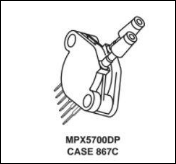
\includegraphics[keepaspectratio=true,scale= 1.5]{figuras/mpx_5700.PNG}
	\caption{ Sensor de Pressão Diferencia}
	\label{SensordePressao}
\end{figure}
A faixa de leitura de pressão é de 15 a 700KPa (2.18 a 101.5psi) com saída analógica de 0.2 a 4.7V. Considerando que a entrada diferencial representa a pressão ambiente, a saída mínima representa este valor. Caso a entrada seja isolada, se obtêm a pressão absoluta da entrada analisada.
Por ser um sensor ativo, a alimentação necessária é por padrão 5V mas permite o correto funcionamento entre 4.75V – 5.25V. Pode-se também utilizar uma alimentação inferior, que em questão será de 3.3V, porém deve-se observar a correspondência com a saída. Tal relação é observada na eq.(3.2).
\begin{equation}
V_{out} = V_{s}*(0.00369 * P + 0.04)+2.5\%V_{out} 	
\end{equation}
Sendo P a pressão que se deseja obter, Vout a tensão de saída do sensor e Vs a tensão de alimentação.
A sensibilidade do sensor é definida a partir da variação da saída em tensão em relação à entrada. Que consiste em 6.4mV a cada KPa de entrada.
Quanto às características físicas, possui 6 pinos, porém somente 3 são utilizados, que são correspondentes à alimentação, referência e saída. As entradas são duas, diferenciais, sendo uma a referência absoluta e a outra a que se deseja ser analisada.
Sua curva característica pode ser observada na Figura \ref{Curva} . 
\begin{figure}[h!]
	\centering
	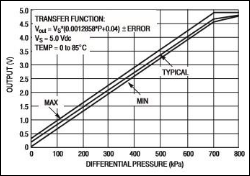
\includegraphics[keepaspectratio=true,scale= 1.5]{figuras/curva_carc.PNG}
	\caption{ Curva característica do MPX5700.}
	\label{Curva}
\end{figure}
\subsection{Compensador de Junta Fria e Conversor A/D MAX6675}
O MAX6675 realiza a compensação de junta fria necessária para ler com coerência a diferença de tensão na saída do termopar. Também converte para digital esta tensão diferencial de saída com resolução de 12 bits e permite um passo de 0.25 graus Celsius dentro da faixa de 0 a 700 graus com precisão. 
É especificamente utilizado em aplicações microcontroladas e acoplado a termopares tipo K. Sua ligação física é mostrada na Figura \ref{Circuito}, sendo compatível com o microcontrolador a ser utilizado neste projeto.
\begin{figure}[h!]
	\centering
	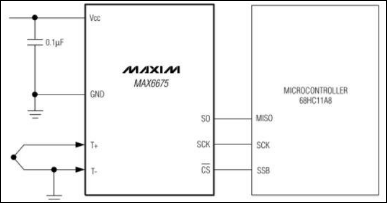
\includegraphics[keepaspectratio=true,scale= 0.9]{figuras/sensor_temp.PNG}
	\caption{ Circuito para Sensor de Temperatura.}
	\label{Circuito}
\end{figure}
A resolução do sensor associada ao circuito é de 41 $\mu$V por grau Celsius com um erro máximo de 3 graus por leitura. Tornando então a ideia de uma média das leituras viável para obter o valor mais próximo ao real. Esta leitura leva em consideração que a temperatura da junta na extremidade do termopar se encontra a mesma da temperatura ambiente. Caso contrário deve-se subtrair estes valores e multiplicar pelo valor da saída para compensar o erro na leitura.
Alimentado com 3.3V, considerando a possibilidade de 3 – 5V, a o erro pode chegar até 5 estados lógicos e a constante de conversão do termopar é de 10.25 $\mu$V por estado lógico.
Uma visão interna do C.I. pode ser observada na Figura \ref{Circuitomax} .
\begin{figure}[h!]
	\centering
	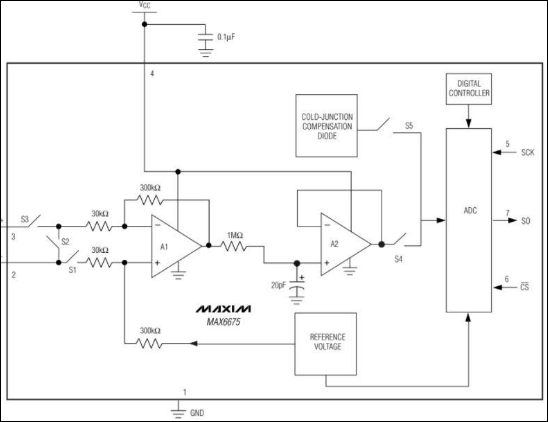
\includegraphics[keepaspectratio=true,scale= 0.7]{figuras/max6675.PNG}
	\caption{ Circuito interno max6675.}
	\label{Circuitomax}
\end{figure}
\subsection{Termopar tipo K}
O termopar é um sensor de temperatura simples e de vasta aplicação. Consiste basicamente em dois metais distintos de duas junções e unidos em uma das pontas. Quando há diferença de temperatura entre a junção unida e a separada gera uma diferença de tensão entre as duas pontas separadas.
Tipo K define o tipo de material que, neste caso permite leituras de temperatura de aproximadamente -270 a 1200 graus Celcius.
Todos os componentes obtidos são apresentados nos anexos deste documento. 

\section{Procedimentos para Funcionamento dos Sensores}
Para iniciar os testes com os sensores um protótipo do circuito final impresso é projetado na protoboard para certificar que tudo está funcionando como esperado e realizar alguns ajustes. Após concluída esta etapa o acoplamento dos sensores no motor deve ser realizado e por fim o circuito final desenvolvido para que possa então permanecer em funcionamento permanente na bancada.
Abaixo serão apresentados alguns dos avanços já realizados:
\begin{itemize}
\item Foram adquiridos os sensores de pressão, de temperatura, os capacitores necessários para montagem do circuito e o circuito integrado para condicionar e converter o sinal de saída do termopar de analógico para digital.
\item Com o sensor de pressão foi montado o circuito mostrado na Figura \ref{Circuitompx} e testada a variação de tensão na saída com o auxílio de uma seringa. Observando corretamente a variação linear de tensão de saída, que é regida pela eq. (3.2)
\begin{figure}[h!]
	\centering
	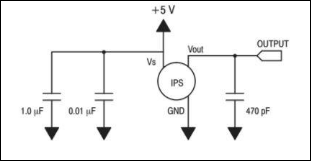
\includegraphics[keepaspectratio=true,scale= 1.5]{figuras/circuito_mpx.PNG}
	\caption{ Circuito para MPX5700.}
	\label{Circuitompx}
\end{figure}
\item Este sensor diferencial de pressão possui saída analógica, necessitando então de uma conversão para correta apresentação digital dos seus dados. Conversão não necessária para o sensor de temperatura visto que o sinal adquirido será digital.
\item Após a conversão dos dados é necessário transmitir os mesmos para introduzi-los à interface com o usuário e assim realizar a análise dos dados adquiridos.
\end{itemize}
Tanto a conversão quanto a transmissão foram realizadas com sucesso seguindo exatamente o fluxograma da Figura \ref{Fluxograma1}.
\begin{figure}[h!]
	\centering
	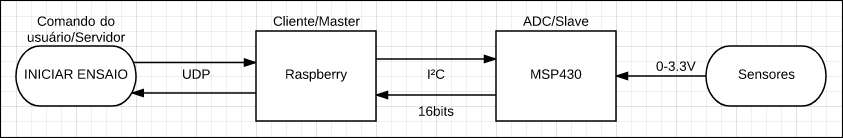
\includegraphics[keepaspectratio=true,scale= 0.7]{figuras/diagrama_de_transmissao.PNG}
	\caption{ Fluxograma de conversão e transmissão de dados dos sensores.}
	\label{Fluxograma1}
\end{figure}
Os procedimentos futuros para que se possa concluir o objetivo de coletar, tratar e apresentar os sinais relevantes, obtidos do motor, para análise de seu funcionamento são:
\begin{itemize}
	\item Realizar testes de funcionamento do termopar com o circuito integrado acoplado;
	\item Calibrar os sensores;
	\item Ler os valores de saída dos sensores a partir do microcontrolador;
	\item Calcular a conversão de tensão para as grandezas que se deseja obter;	
\end{itemize}
\section{Procedimentos de Controle de Partida do Motor}
O sistema de controle de acionamento e aceleração do motor é composto principalmente pelo sistema de comunicação entre raspberry e msp430 via I$^{2}$C. O fluxo do sistema parte do acionamento do usuário pela aplicação que inicia um comando de uma requisição de escrita da raspberry em um registrador da msp430, se o valor enviado for igual o valor pré-definido para executar a operação uma das portas digitais recebe nível alto acionando o optoacoplador que sequencialmente aciona a contatora para acionar o motor de partida. Quando o motor inicia a combustão os eixos do motor são acionados gerando então pulsos no sensor de giro, este sensor é conectado a uma porta de entrada da msp430 para definir o início da combustão, quando esta porta recebe algum valor diferente de 0V a msp430 corta a alimentação do motor de partida, desacionando a contatora.
\begin{figure}[h!]
	\centering
	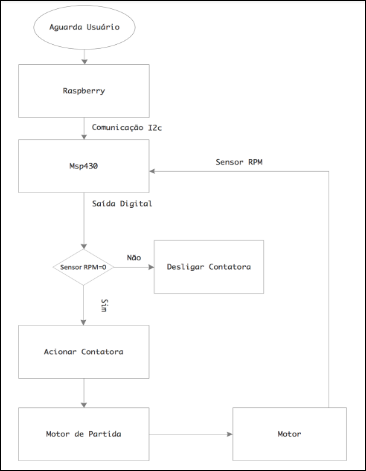
\includegraphics[keepaspectratio=true,scale= 1.5]{figuras/fluxograma1.PNG}
	\caption{ Fluxograma de Acionamento do Motor}
	\label{ Fluxograma de Acionamento do Motor}
\end{figure}
Para o controle de aceleração o sistema será binário (aceleração total ou totalmente desacelerado). Assim como o sistema de acionamento, o fluxo do sistema de aceleração parte de um comando do usuário que inicia uma requisição de escrita da raspberry na msp430 se o valor de escrita for igual ao valor pré-definido, a msp430 configura uma de suas portas para uma saída PWM(\textit{Pulse Width Modulation}) que habilita a rotação do servomotor em 90$^{o}$ fazendo a abertura total da válvula borboleta. A desacelaração é realizada pelo mesmo comando do usuário, seguindo o mesmo fluxo descrito.
\begin{figure}[h!]
	\centering
	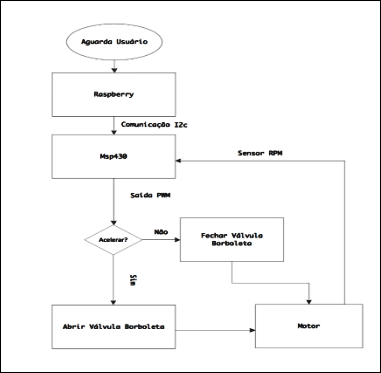
\includegraphics[keepaspectratio=true,scale= 1.5]{figuras/fluxograma2.PNG}
	\caption{ Fluxograma de Aceleração/Desaceleração do Motor}
	\label{ Fluxograma de Aceleração/Desaceleração do Motor}
\end{figure}
\section{Procedimentos para Conversão e Transmissão dos dados}
Ao total são 6 sensores analógicos que necessitam de conversão para realizar o tratamento e disposição digital. O sistema de conversão e transmissão de dados são posteriores ao condicionamento dos sinais.
O msp430 possui 8 canais para conversão ADC(\textit{Analogic to Digital Conversor}) conversão múltiplas. Para o projeto, serão utilizados 6 canais, tendo em vista o número de sensores analógicos presentes no projeto. O conversor ADC foi configurado para atuar no modo de múltiplas conversões que dessa forma, inicia a conversão no canal mais significativo (no caso canal A6 - 1 por sensor) até o conversor menos significativo (A0). Além disso, o conversor possui uma resolução de 10 bits. Como os valores de tensão estão em uma faixa entre [0, 3.3] volts a precisão do conversor é dado por:
\begin{equation}
precisão = \frac{3.3}{2^{10}}
\end{equation}
Os valores de tensão convertidos em palavras binárias apresentam valores inteiros entre 0 e 1023, onde 1023 representa a tensão máxima de 3.3V.
O sistema de comunicação I$^{2}$C realiza a transmissão de 1 byte por vez, como o conversor é de 10 bits, a transmissão de uma palavra referente a um sensor necessita então de dois bytes. Portanto, se cada 2 bytes representam um valor de um sensor, portanto 6 sensores representam um total de:
\begin{equation}
total de bytes por conversão = (2*6)bytes = 12bytes
\end{equation}
O conversor é configurado para realizar continuamente as conversões dos 6 canais, assim que o usuário executa o comando “START” que aciona o motor. A conversão destes 6 canais são armazenados em uma variável de tamanho 12 bytes, armazenando o valor das 6 conversões.
Quando o usuário executa o comando “INICIAR ENSAIO” inicia-se a comunicação I$^{2}$C entre raspberry e msp430. A taxa de transmissão é configurada através de um timer que configura a taxa de transmissão em 100Kbits/s ou então 12.5Kbytes/s. Esta taxa de transmissão garante que não haja violação de \textit{setup} ou violação de \textit{hold}, fazendo com que não haja perda de informação ou encavalamento de bits.
Como a variável que contém o valor de todos os sensores possui tamanho de 12 bytes o tempo estimado para transmissão é dado por:
\begin{equation}
tempo de transmissão = \frac{12bytes}{12.5Kbytes/s} = 960 \mu s
\end{equation}
Este é o tempo para transmitir a informação, porém na configuração I$^{2}$C ainda são transmitidos, condição de start, condição de parada, endereço, dados, condição de parada, totalizando um total de 24 bits ou 3 bytes. Portanto para transmitir todos os valores são transmitidos um total de 3*12bytes = 36 bytes, portanto o tempo total de transmissão é dado por:
\begin{equation}
tempo total de transmissão = \frac{36bytes}{12.5Kbytes/s} = 2.88 ms
\end{equation}
A taxa de conversão dos sensores obedecendo o critério de Nyquist é configurado para uma taxa de 1KHz ou 1000 amostras/s sabendo que o sinal de maior frequência possui frequência de 256 Hz.
\\%colocar fig da simulação de transmissão
\begin{figure}[h!]
	\centering
	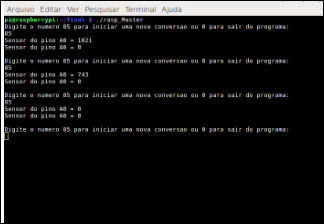
\includegraphics[keepaspectratio=true,scale= 1.5]{figuras/Simulacao_I2C.PNG}
	\caption{Simulação da leitura, conversão e transmissão de dois sensores analógicos}
	\label{Simulação}
\end{figure}
Sempre que a raspberry envia o número decimal 85 é realizada uma conversão e transmissão de todos os sensores conectados aos canais de conversão da MSP430. No exemplo da Figura \ref{Simulação} a apenas variou-se o valor do sensor 1 mantendo o valor do sensor 2 em nível 0 para confirmar a medição.
